%%%%%%%%%%%%%%%%%%%% author.tex %%%%%%%%%%%%%%%%%%%%%%%%%%%%%%%%%%%
%
% sample root file for your "contribution" to a proceedings volume
%
% Use this file as a template for your own input.
%
%%%%%%%%%%%%%%%% Springer %%%%%%%%%%%%%%%%%%%%%%%%%%%%%%%%%%


\documentclass{svproc}
%
% RECOMMENDED %%%%%%%%%%%%%%%%%%%%%%%%%%%%%%%%%%%%%%%%%%%%%%%%%%%
%

% to typeset URLs, URIs, and DOIs
\usepackage[bottom]{footmisc}
\usepackage{url}
\usepackage{booktabs}
\usepackage{amsmath}
\usepackage{graphicx}
\usepackage{booktabs}          % \toprule, \midrule, \bottomrule
\usepackage{array}             % >{\raggedright\arraybackslash}p{...} columns
\usepackage{multirow}          % only if you use \multirow
\usepackage{algorithm}         % algorithm float
\usepackage{algorithmicx}
\usepackage{algpseudocode}     % \Require, \ForAll, \State, \Comment, \Return
\def\UrlFont{\rmfamily}

\begin{document}
\mainmatter              % start of a contribution
%
\title{Parameter-Efficient Adaptation of Multilingual Transformers for Telugu Abusive Comment Detection}
%
\titlerunning{Parameter-Efficient Adaptation for Telugu Abusive Language Detection}  % abbreviated title (for running head)
%
\author{Venkataramana Battula \and Durga Prasad}
%
\authorrunning{V. Battula and D. Prasad} % abbreviated author list (for running head)
%
\institute{Department of Computer Science and Engineering\\
\email{\{vbattula, dprasad\}@academic.edu}}

\maketitle              % typeset the title of the contribution
\begin{abstract}
Abusive comment detection in low-resource Indian languages is hampered by limited compute, character-level obfuscation, and weakly controlled evaluations of adaptation strategies. This study examines parameter-efficient fine-tuning (PEFT) for Telugu abusive comment detection on the Telugu subset of the Multilingual Abusive Comment Detection (MACD) corpus. Full fine-tuning, LoRA, DoRA, and AdaLoRA are evaluated with XLM-RoBERTa, MuRIL, multilingual BERT, and IndicBERT v2, alongside a TF-IDF linear SVM baseline. Experiments use three seeds, validation macro-F1 for model selection, paired bootstrap intervals, and McNemar tests on identical test instances. LoRA on XLM-RoBERTa reaches a test macro-F1 of 0.9035, close to the 0.9057 of full fine-tuning, while updating 0.32\% of parameters and using about one-third of the GPU memory; the difference is not significant. DoRA gives no measurable gain, and AdaLoRA performs significantly worse. The SVM baseline reaches 0.9029, statistically indistinguishable from the adapted transformers. A rule-based normalizer covering 20 obfuscation patterns raises mean accuracy from about 0.71 to 0.86. Advertisement-like template comments make up roughly 15\% of abusive comments and inflate scores by about 0.8 points without changing rankings. Finally, an allow, review, and block pipeline is demonstrated with a 3.4 MB LoRA adapter. The findings support PEFT for resource-efficient Telugu moderation and stress robust evaluation.
\keywords{abusive language detection, Telugu, low-resource languages, parameter-efficient fine-tuning, LoRA, DoRA, AdaLoRA, XLM-RoBERTa, calibration}
\end{abstract}

\section{Introduction}
Abusive comments are a persistent problem on social platforms, and moderation for Indian languages is harder than for English because labeled data, pretrained models and tooling are less mature. Telugu is spoken by more than 80 million people, yet it has far fewer public benchmarks than English. Early work framed the task as classification of short texts with lexical features \cite{waseem2016,davidson2017}, and surveys document the shift towards neural models \cite{schmidt2017}. Pretrained transformer encoders \cite{vaswani2017,devlin2019bert} now provide strong accuracy, but fully fine-tuning a 278-million-parameter model for every language, task or domain is costly in memory, storage and time. Parameter-efficient fine-tuning (PEFT) keeps the pretrained weights frozen and trains small additional modules \cite{houlsby2019,hu2022lora}, which makes per-task adapters of a few megabytes practical.

The closest prior work applies LoRA to hate speech detection in another low-resource language \cite{kaunang2026indo}, but without a full fine-tuning reference, competing adaptation methods, a classical baseline, seed variance or significance testing, and without examining robustness or deployment. Whether parameter-efficient adaptation is a sound choice for Telugu, and at what cost, therefore remains open. 

\begingroup
\renewcommand{\labelitemi}{$\bullet$}
This paper makes the following contributions:
\begin{itemize}
    \item A comparison of full fine-tuning, LoRA, DoRA, and AdaLoRA using four multilingual transformer models on the Telugu MACD dataset \cite{gupta2022macd}, considering three random seeds, model performance, training time, memory usage, and model size.
    \item A statistical comparison of model results using bootstrap and McNemar tests, along with a reproduction of the published LoRA method \cite{kaunang2026indo} and an improved configuration.
    \item An evaluation of a TF-IDF baseline and input-guard ablation to understand the contributions of traditional machine learning, transformer models, and adaptation methods to classification performance.
    \item A deployment pipeline that includes temperature scaling, review thresholds, and INT8 model export, with an evaluation of the limitations of quantized models.
    \item An analysis of model errors and dataset characteristics, showing that many errors are shared across different models and that some abusive comments follow advertisement-like patterns.
\end{itemize}
\endgroup

The remainder of the paper is organized as follows. Section~\ref{sec:related} reviews related work and identifies the research gaps. Section~\ref{sec:method} describes the data, models, training protocol and deployment pipeline. Section~\ref{sec:results} reports and discusses the results, and Section~\ref{sec:concl} concludes.

\section{Background}
\label{sec:related}
Abusive language detection is an important research problem in natural language processing (NLP), particularly for social media content characterized by informal expressions, spelling variations, and code-mixing. Gupta et al.~\cite{gupta2022macd} introduced the Multilingual Abusive Comment Detection (MACD) dataset, which contains approximately 150,000 comments across five Indic languages. The Telugu subset provides a benchmark for binary abusive language classification. However, detecting abusive expressions in Telugu remains challenging because of linguistic variation, contextual ambiguity, and the use of non-standard writing conventions in social media communication.

Pretrained multilingual transformer models have improved text classification by learning contextual representations from large-scale corpora. Multilingual BERT (mBERT), introduced by Devlin et al.~\cite{devlin2019bert}, was pretrained on Wikipedia text in 104 languages. XLM-RoBERTa (XLM-R), proposed by Conneau et al.~\cite{conneau2020xlmr}, uses large-scale CommonCrawl data to improve cross-lingual representation learning. MuRIL, developed by Khanuja et al.~\cite{khanuja2021muril}, was designed specifically for Indian languages and incorporates transliterated text in its pretraining. IndicBERT v2, described by Doddapaneni et al.~\cite{doddapaneni2023indicbert}, uses the IndicCorp v2 corpus to support language understanding across 24 Indic languages. These models differ in their pretraining data, language coverage, and treatment of Indian-language text, making their comparative evaluation relevant to Telugu abusive language detection. In the present study, IndicBERT v2 is considered because the original IndicBERT checkpoint was not accessible in the experimental environment.

Full fine-tuning updates all trainable parameters of a pretrained transformer and can require substantial computational resources. Parameter-efficient fine-tuning (PEFT) methods address this limitation by adapting pretrained models while reducing the number of trainable parameters. Houlsby et al.~\cite{houlsby2019} introduced adapter modules that are inserted between pretrained network layers. Prefix tuning and prompt tuning provide alternative approaches by learning additional continuous representations that influence model predictions~\cite{li2021prefix,lester2021prompt}. Aghajanyan et al.~\cite{aghajanyan2021intrinsic} demonstrated that effective fine-tuning can operate within a lower-dimensional parameter space than the full model parameterization.

Low-Rank Adaptation (LoRA), introduced by Hu et al.~\cite{hu2022lora}, freezes pretrained weights and learns low-rank updates to selected weight matrices. DoRA extends this approach by decomposing weight updates into magnitude and direction components~\cite{liu2024dora}. AdaLoRA dynamically allocates the rank of low-rank updates according to parameter importance~\cite{zhang2023adalora}. QLoRA combines low-bit quantization with LoRA to reduce memory requirements during fine-tuning~\cite{dettmers2023qlora}, whereas $(IA)^3$ scales selected internal activations using learned vectors~\cite{liu2022ia3}. Implementations of these and other adaptation techniques are available through the Parameter-Efficient Fine-Tuning library~\cite{mangrulkar2022peft}. Although these methods reduce the computational cost of model adaptation, their relative effectiveness can depend on the pretrained backbone, dataset characteristics, and training configuration. Therefore, a controlled comparison with full fine-tuning is necessary to determine whether parameter-efficient adaptation provides an appropriate trade-off between predictive performance and computational efficiency for Telugu abusive language detection.

The reliability of abusive language detection systems depends not only on their performance on unmodified test data but also on their sensitivity to variations in the input text. Hosseini et al.~\cite{hosseini2017} demonstrated that character-level modifications can alter the predictions of toxicity classifiers. Similarly, Gr\"ondahl et al.~\cite{grondahl2018} investigated vulnerabilities in machine learning-based hate speech detection systems and highlighted the susceptibility of such systems to adversarial perturbations. These findings motivate the evaluation of character substitutions, inserted characters, spelling variations, and other text transformations that may preserve the intended meaning while changing the model input.

Such robustness concerns are particularly relevant to Telugu social media text, where users may employ informal spellings, transliterated expressions, and combinations of Telugu and English. A classifier that performs well on an unmodified test set may still be sensitive to these variations. Evaluating prediction changes under controlled text modifications can therefore provide additional evidence about model reliability. Furthermore, input guards may help identify or restrict selected suspicious inputs, but their effectiveness must be assessed independently rather than assumed to provide complete protection against adversarial attacks.

Recent research has also investigated parameter-efficient adaptation for abusive and hate speech detection in languages other than Telugu. Kaunang et al.~\cite{kaunang2026indo} applied LoRA to IndoBERT for Indonesian hate speech detection using data from Instagram, Twitter, and news portals. Their study examines multi-domain classification and the use of data augmentation to address limited data availability in one of the domains. This work illustrates the potential of PEFT for adapting language-specific transformer models to social media classification tasks. However, its primary focus is LoRA-based adaptation of IndoBERT for Indonesian text, rather than a controlled comparison of multiple PEFT methods and multilingual transformer backbones for Telugu abusive language detection.

Despite progress in multilingual classification, several aspects remain important for the present research problem. First, the relative performance of full fine-tuning, LoRA, DoRA, and AdaLoRA across different transformer backbones requires systematic evaluation on Telugu abusive language data. Second, comparisons should consider variation across random seeds and use appropriate statistical procedures to assess whether observed performance differences are significant. Third, the effect of deliberate text modifications on model predictions requires explicit evaluation rather than relying solely on clean-test performance. Finally, calibration, quantization, and potential dataset artifacts are relevant to assessing model reliability and deployment suitability. These issues motivate a unified experimental framework that examines predictive performance, robustness, and computational considerations within the same Telugu classification setting.

To investigate these issues, the present study compares full fine-tuning with LoRA, DoRA, and AdaLoRA using four transformer backbones: mBERT, XLM-R, MuRIL, and IndicBERT v2. A TF-IDF-based linear Support Vector Machine (SVM) is included as a classical machine learning baseline. Model performance is evaluated across multiple random seeds, with bootstrap confidence intervals used to quantify uncertainty and McNemar's test used for paired comparisons of classification errors where its assumptions are satisfied. Validation-based model selection is employed to reduce the risk of selecting configurations using test-set results.

Beyond standard classification performance, robustness is investigated using 20 text-modification attacks and an input guard. Calibration analysis examines the reliability of predicted probabilities, while INT8 quantization is evaluated as a potential means of reducing inference resource requirements. The study also investigates template-related data artifacts that could influence evaluation results. Together, these experiments provide a structured assessment of parameter-efficient adaptation, classification robustness, and practical deployment considerations for Telugu abusive language detection. The contribution lies in the systematic evaluation of these complementary aspects within the specified experimental setting, rather than in claiming that any individual adaptation method or evaluation technique is itself new.

\section{Methodology}
\label{sec:method}
\subsection{Data and preprocessing}
Rows with missing fields and exact duplicates within each split were removed, and comments of the validation and test splits that also occur verbatim in the training split were then dropped (2 and 3 comments, respectively). Table~\ref{tab:data} gives the resulting sizes. The released files use 0 for abusive and 1 for non-abusive; this was verified against the upstream release and remapped to 1 = abusive throughout. Text is Unicode-normalized (NFC), URLs and mentions are masked and whitespace is collapsed; punctuation, emoji and repeated characters are kept, because they can carry abuse signals. The lowercasing and symbol stripping used for Indonesian text in \cite{kaunang2026indo} is not applied.

\begin{table}[t]
\caption{Telugu MACD dataset splits after duplicate removal.}
\label{tab:data}
\centering
\begin{tabular}{lrrrr}
\toprule
Split & Comments & Abusive & Non-abusive & Mean words \\
\midrule
Train      & 23,980 & 12,401 & 11,579 & 12.8 \\
Validation & 2,998  & 1,616  & 1,382  & 13.2 \\
Test       & 2,997  & 1,561  & 1,436  & 12.7 \\
\bottomrule
\end{tabular}
\end{table}

\subsection{Models and training}
All encoders are used as sequence classifiers with a binary head. For PEFT, the base model is frozen, adapters are placed on the attention \texttt{query} and \texttt{value} matrices, and the classification head is trained and saved. Table~\ref{tab:hp} lists the settings; all runs use AdamW \cite{loshchilov2019adamw} with weight decay 0.01, a cosine schedule with 10\% warmup and FP16. Rank $\{4,8,16,32\}$, alpha $\{16,32,64\}$ and learning rate $\{10^{-4},2\times10^{-4},5\times10^{-4}\}$ were searched on MuRIL with one seed, and the selected setting was reused for the other backbones; DoRA and AdaLoRA were therefore not tuned separately. The published recipe of \cite{kaunang2026indo} and a $r=16$, $\alpha=32$ starting configuration were also trained unchanged on XLM-R. Seeds 42, 123 and 2024 were used for every compared configuration. Training used a single 8~GB RTX 4060 Ti with PyTorch 2.6, Transformers \cite{wolf2020transformers} 4.57 and PEFT 0.21.

\begin{table}[t]
\caption{Training settings. ``Published'' denotes the recipe from \cite{kaunang2026indo}, applied unchanged.}
\label{tab:hp}
\centering
\footnotesize
\setlength{\tabcolsep}{3.5pt}
\begin{tabular}{lccc}
\toprule
Setting & This work (PEFT) & Full FT & Published \\
\midrule
Rank $r$ / alpha $\alpha$ & 8 / 64 & -- & 4 / 32 \\
LoRA dropout & 0.05 & -- & 0.1 \\
Target modules & query, value & all & query, value \\
Learning rate & $2\times10^{-4}$ & $2\times10^{-5}$ & $2\times10^{-4}$ \\
Batch size & 16 & 16 & 8 \\
Max length (tokens) & 96 & 96 & 128 \\
Maximum epochs & 10 & 5 & 5 \\
Early stopping & \multicolumn{3}{c}{Patience of 3 epochs on validation macro-F1} \\
\bottomrule
\end{tabular}
\end{table}

\subsection{Classical baseline}
The baseline uses TF-IDF features from character 2--5-grams within word boundaries and word 1--2-grams, with a linear SVM \cite{cortes1995svm} implemented in scikit-learn \cite{pedregosa2011sklearn}. The regularization constant was chosen from $\{0.1,0.3,1,3,10\}$ on validation macro-F1 (the selected value is 0.3).

\subsection{Metrics}
Let TP, FP, FN and TN be the counts of true and false positives and negatives for the abusive class. Then

\begin{align}
P_c &= \frac{TP_c}{TP_c+FP_c}, \label{eq:prec}\\
R_c &= \frac{TP_c}{TP_c+FN_c}, \label{eq:rec}\\
F_{1,c} &= \frac{2P_cR_c}{P_c+R_c}, \label{eq:f1}\\
\text{macro-}F_1 &= \frac{1}{|\mathcal{C}|}\sum_{c\in\mathcal{C}} F_{1,c}, \label{eq:macrof1}\\
\mathrm{ECE} &= \sum_{b=1}^{B}\frac{|S_b|}{n}\,\bigl|\mathrm{acc}(S_b)-\mathrm{conf}(S_b)\bigr|. \label{eq:ece}
\end{align}

where $S_b$ are confidence bins \cite{guo2017calibration}. Macro-F1 weights both classes equally \cite{sokolova2009}. Accuracy, weighted-F1 and the confusion matrix are also reported.

\begin{figure*}[t]
\centering
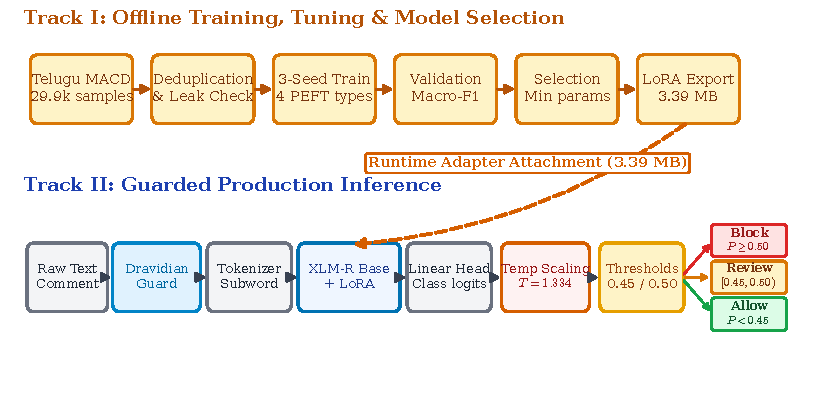
\includegraphics[width=\textwidth]{figures/fig2_system_architecture.pdf}
\caption{Pipeline. Top: experiment and selection path (orange boxes); selection uses validation macro-F1 only and the test set is never used. Bottom: deployed inference path from raw comment to decision. The selected LoRA adapter (dashed arrow) is attached to the frozen XLM-R encoder (blue box); the final decision (green box) is made with two thresholds: a lower threshold of 0.45 routes uncertain comments to human review, while an upper threshold of 0.50 triggers automated blocking, chosen on validation data to achieve a block precision exceeding 0.90.}
\label{fig:arch}
\end{figure*}

\subsection{Selection and statistical testing}
Selection used validation scores only (Algorithm~\ref{alg:select}): configurations with three seeds were ranked by mean validation macro-F1, all configurations within one standard deviation of the best form a tie set, and the member with the fewest trainable parameters is selected. The test set was read once per run for reporting. Differences between the selected model and each alternative were tested on the same 2,997 test comments with a paired bootstrap of the macro-F1 difference (10,000 resamples, 95\% percentile interval \cite{efron1993bootstrap}) and an exact McNemar test \cite{mcnemar1947}, in line with recommended practice \cite{dror2018}. Seeds matter because fine-tuning variance is substantial \cite{dodge2020}. A Bonferroni correction for 11 pairwise comparisons ($\alpha = 0.05 / 11 \approx 0.0045$) was applied when reporting family-wise statistical significance.

\begin{algorithm}[t]
\caption{Model selection procedure. The test set is never used.}\label{alg:select}
\footnotesize
\begin{algorithmic}[1]
\Require configurations $\mathcal{C}$, each trained with seeds $\{42,123,2024\}$
\ForAll{$c \in \mathcal{C}$ with three completed seeds}
  \State $\mu_c, \sigma_c \leftarrow$ mean and sample std of validation macro-F1
\EndFor
\State $c^\star \leftarrow \arg\max_c \mu_c$
\State $\mathcal{T} \leftarrow \{c : \mu_c \ge \mu_{c^\star} - \sigma_{c^\star}\}$ \Comment{tie set}
\State $\hat{c} \leftarrow$ member of $\mathcal{T}$ with the fewest trainable parameters
\State \Return the seed of $\hat{c}$ with the highest validation macro-F1
\end{algorithmic}
\end{algorithm}

\subsection{Deployment pipeline}
At inference (Fig.~\ref{fig:arch}), text passes through an input guard that removes zero-width characters, separators inserted inside words, spaced-out letters and stretched letters, then through the classifier. Logits are rescaled with a temperature fitted on validation \cite{guo2017calibration} (a Platt scaling \cite{platt1999} is used for the SVM), and two thresholds on the abuse probability give an allow, review or block decision. The thresholds are chosen on validation to maximize block recall subject to block precision of at least 0.9. Words that drive a decision are found by occlusion, removing each word and measuring the drop in abuse probability \cite{zeiler2014}. The adapter is merged into the base model and exported to ONNX with dynamic INT8 weights \cite{jacob2018}.

\section{Results and Discussion}
\label{sec:results}
\subsection{Accuracy and cost}
Table~\ref{tab:main} gives mean and standard deviation over three seeds. Full fine-tuning, LoRA and DoRA on XLM-R and MuRIL lie between 0.9005 and 0.9057 test macro-F1, IndicBERT v2 LoRA reaches 0.9017 and mBERT LoRA 0.8946, and AdaLoRA is lowest (0.8891 on XLM-R, 0.8945 on MuRIL). The selected XLM-R LoRA model trains 887,042 parameters (0.32\% of 278.0 million) and peaks at 1.75~GB of GPU memory against 5.35~GB for full fine-tuning, with a 3.4~MB adapter in place of a 1.1~GB checkpoint. Figure~\ref{fig:front} plots accuracy against the number of trained parameters, and Fig.~\ref{fig:cost} compares memory and time.

\begin{table*}[t]
\caption{Validation and test macro-F1 (mean $\pm$ standard deviation, three seeds), trained parameters, peak GPU memory and training time. Model selection used validation only. Times were measured with other load on the GPU and are indicative; rows marked ``5 ep.'' were trained for five epochs, so their times are not directly comparable to the others. The SVM baseline is a single run on CPU only.}
\label{tab:main}
\centering
\footnotesize
\setlength{\tabcolsep}{3pt}
\resizebox{\textwidth}{!}{%
\begin{tabular}{llccrrr}
\toprule
Backbone & Method & Val macro-F1 & Test macro-F1 & Params (M) & GPU (GB) & Time (s) \\
\midrule
XLM-R & Full fine-tuning & $\mathbf{0.9040}\pm0.0011$ & $\mathbf{0.9057}\pm0.0033$ & 278.0 & 5.35 & 1564 \\
XLM-R & LoRA (selected) & $0.9035\pm0.0043$ & $0.9035\pm0.0033$ & 0.887 & 1.75 & 774 \\
XLM-R & DoRA & $0.9027\pm0.0011$ & $0.9055\pm0.0009$ & 0.905 & 1.89 & 1125 \\
XLM-R & AdaLoRA & $0.8855\pm0.0015$ & $0.8891\pm0.0013$ & 1.035 & 1.76 & 1618 \\
XLM-R & LoRA, $r{=}4,\alpha{=}32$, 5 ep.\ \cite{kaunang2026indo} & $0.8957\pm0.0014$ & $0.8985\pm0.0018$ & 0.740 & 1.59 & 706 \\
XLM-R & LoRA, $r{=}16,\alpha{=}32$, 5 ep. & $0.8933\pm0.0002$ & $0.8953\pm0.0033$ & 1.182 & 1.92 & 454 \\
\midrule
MuRIL & Full fine-tuning & $0.9035\pm0.0023$ & $0.9049\pm0.0028$ & 237.6 & 4.59 & 1250 \\
MuRIL & LoRA & $0.9026\pm0.0020$ & $0.9052\pm0.0030$ & 0.296 & 1.59 & 718 \\
MuRIL & DoRA & $0.8984\pm0.0013$ & $0.9005\pm0.0030$ & 0.315 & 1.73 & 1078 \\
MuRIL & AdaLoRA & $0.8892\pm0.0030$ & $0.8945\pm0.0003$ & 0.444 & 1.60 & 1282 \\
\midrule
IndicBERT v2 & LoRA & $0.8985\pm0.0014$ & $0.9017\pm0.0039$ & 0.296 & 1.75 & 673 \\
mBERT & LoRA & $0.8999\pm0.0010$ & $0.8946\pm0.0015$ & 0.296 & 1.37 & 680 \\
\midrule
-- & TF-IDF + linear SVM (one run) & 0.8993 & 0.9029 & -- & -- & -- \\
\bottomrule
\end{tabular}}
\end{table*}

\begin{figure}[t]
\centering
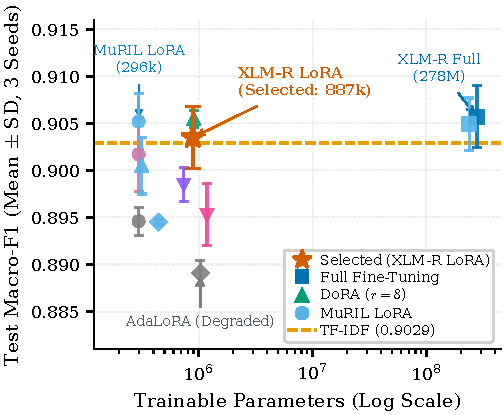
\includegraphics[width=\columnwidth]{figures/fig3_parameter_efficiency_frontier.pdf}
\caption{Test macro-F1 against trained parameters (mean of three seeds; XLM-R and MuRIL points; LoRA also shows IndicBERT v2 and mBERT). Almost all methods sit on one horizontal band, except AdaLoRA; the dashed line is the TF-IDF baseline.}
\label{fig:front}
\end{figure}

\begin{figure}[t]
\centering
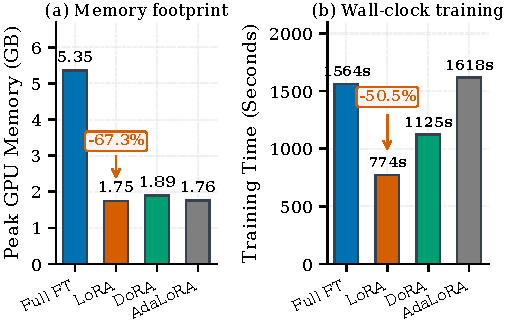
\includegraphics[width=\columnwidth]{figures/fig4_computational_cost.pdf}
\caption{Cost on XLM-R (mean of three seeds). LoRA uses about one third of the memory of full fine-tuning; AdaLoRA is the slowest. Times include other GPU load and are indicative.}
\label{fig:cost}
\end{figure}

\subsection{Per-class metrics}
Table~\ref{tab:perclass} breaks the scores down by class. LoRA is more cautious than full fine-tuning: its precision on abusive comments is higher (0.929 against 0.914) but its recall is lower (0.883 against 0.905), so it misses more abuse and flags fewer innocent comments. Figure~\ref{fig:cm} shows the confusion matrix of the selected run. If missing abuse is the costlier error, full fine-tuning, DoRA, or a lower decision threshold on LoRA is the safer choice.

\begin{table*}[t]
\caption{Per-class test metrics (mean over three seeds, except the single-run SVM). P, R and F1 (abusive) are precision, recall and F1 for the abusive class; F1 (non-abusive) is the F1 of the other class. Macro-F1 is the mean of the two class F1 scores.}
\label{tab:perclass}
\centering
\footnotesize
\setlength{\tabcolsep}{4pt}
\resizebox{\textwidth}{!}{%
\begin{tabular}{lccccccc}
\toprule
Model & Acc. & P (abus.) & R (abus.) & F1 (abus.) & F1 (non-abus.) & Macro-F1 & Weighted-F1 \\
\midrule
XLM-R full fine-tuning & 0.906 & 0.914 & \textbf{0.905} & \textbf{0.909} & 0.902 & 0.906 & 0.906 \\
XLM-R LoRA (selected) & 0.904 & \textbf{0.929} & 0.883 & 0.905 & 0.902 & 0.904 & 0.904 \\
XLM-R DoRA & 0.906 & 0.922 & 0.894 & 0.908 & 0.903 & 0.906 & 0.906 \\
XLM-R AdaLoRA & 0.889 & 0.904 & 0.881 & 0.892 & 0.886 & 0.889 & 0.889 \\
\midrule
MuRIL full fine-tuning & 0.905 & 0.919 & 0.897 & 0.908 & 0.902 & 0.905 & 0.905 \\
MuRIL LoRA & 0.905 & 0.919 & 0.898 & 0.908 & 0.902 & 0.905 & 0.905 \\
MuRIL DoRA & 0.901 & 0.913 & 0.895 & 0.904 & 0.897 & 0.900 & 0.901 \\
MuRIL AdaLoRA & 0.895 & 0.914 & 0.881 & 0.897 & 0.892 & 0.895 & 0.895 \\
\midrule
IndicBERT v2 LoRA & 0.902 & 0.917 & 0.892 & 0.904 & 0.899 & 0.902 & 0.902 \\
mBERT LoRA & 0.895 & 0.917 & 0.877 & 0.897 & 0.893 & 0.895 & 0.895 \\
\midrule
TF-IDF + linear SVM (one run) & 0.903 & \textbf{0.929} & 0.882 & 0.904 & 0.901 & 0.903 & 0.903 \\
\bottomrule
\end{tabular}}
\end{table*}

\begin{figure}[t]
\centering
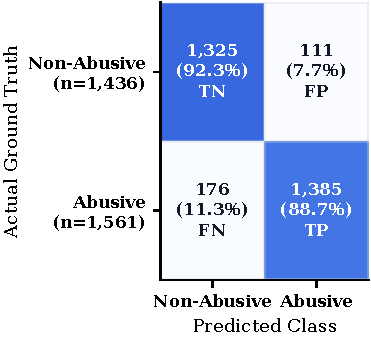
\includegraphics[width=0.7\columnwidth]{figures/fig5_confusion_matrix.pdf}
\caption{Confusion matrix of the selected model (seed 2024) on 2,997 test comments; percentages are row-normalized.}
\label{fig:cm}
\end{figure}

\subsection{Where the models fail}
Table~\ref{tab:slices} reports test macro-F1 on slices of the test set for the selected model, full fine-tuning and the TF-IDF baseline (one seed each). Comments with emoji are the easiest (about 0.93). The transformers hold up better than TF-IDF on long comments of more than 20 words (0.902 and 0.911 against 0.887), which is consistent with their use of wider context, but the slices are small and single-seed, so these differences are indicative only.

\begin{table}[t]
\caption{Test macro-F1 on slices of the test set (one seed per system). ``Latin letters'' marks comments with any Roman-script character.}
\label{tab:slices}
\centering
\footnotesize
\setlength{\tabcolsep}{4pt}
\begin{tabular}{lrcccc}
\toprule
Slice & $n$ & Abusive & LoRA & Full FT & TF-IDF \\
\midrule
1--5 words & 814 & 0.40 & 0.897 & 0.900 & 0.901 \\
6--10 words & 976 & 0.47 & 0.903 & 0.910 & 0.907 \\
11--20 words & 729 & 0.59 & 0.894 & 0.898 & 0.888 \\
Over 20 words & 478 & 0.73 & 0.902 & 0.911 & 0.887 \\
Contains emoji & 1,178 & 0.53 & 0.929 & 0.934 & 0.925 \\
Contains Latin letters & 616 & 0.65 & 0.910 & 0.900 & 0.908 \\
Telugu script only & 2,381 & 0.49 & 0.901 & 0.910 & 0.900 \\
\bottomrule
\end{tabular}
\end{table}

The errors are strongly shared. Comparing single runs (seed 2024 for the transformers), of the 287 test errors of the selected model, 122 (42.5\%) are also made by full fine-tuning, DoRA, MuRIL LoRA and TF-IDF; 86 of these 122 carry the abusive label and 36 the non-abusive label. The selected model's errors overlap with those of full fine-tuning (Jaccard 0.60) more than with those of TF-IDF (0.45). Had at least one of the five systems been chosen correctly for every comment, accuracy would be 0.959, an upper bound that suggests some room for combining models. The selected model misses abuse more often than it raises false alarms (178 false negatives against 112 false positives after calibration and the input guard), and 101 of its 290 errors in the deployed pipeline have a confidence of at least 0.9. Comments that every system gets wrong with high confidence are candidates for label noise or for abuse that needs context; they were not re-annotated.

\subsection{Template artifacts in the data}
The word-frequency analysis of the training split showed a group of terms that occur almost only in abusive comments and are not abusive words: the Telugu words for ``problems'', ``for any problem'', ``progeny'', ``husband and wife'', a term for love spells, and formal phrases such as ``will be done''. They come from advertisement-like posts for astrology and spell services. Every comment containing one of these markers was flagged (Table~\ref{tab:template}). About 15\% of abusive comments in each split are such posts, and almost all flagged posts carry the abusive label. All three systems classify them with 99.6\% accuracy. Removing them from the test set lowers macro-F1 by about 0.7 to 0.8 points for every system (seed 2024; selected LoRA 0.8964, full fine-tuning 0.9019, TF-IDF 0.8949), so the comparison between systems does not change, but reported scores on this corpus are inflated by an easy, template-driven subset. Whether such posts should count as abusive is a labeling decision of the source corpus, which was not revisited.

\begin{table}[t]
\caption{Advertisement-like template posts flagged by seven marker strings (listed in Section~\ref{sec:template_markers}). ``Share of abusive'' is the number of flagged posts labeled abusive divided by all abusive posts in that split.}
\label{tab:template}
\centering
\footnotesize
\setlength{\tabcolsep}{4pt}
\begin{tabular}{lrrrr}
\toprule
Split & Flagged & Abusive & Non-abusive & Share of abusive (\%) \\
\midrule
Train      & 1,935 & 1,928 & 7 & 15.5 \\
Validation & 267   & 264   & 3 & 16.3 \\
Test       & 227   & 227   & 0 & 14.5 \\
\bottomrule
\end{tabular}
\end{table}

\subsection{Training behavior}
Figure~\ref{fig:curve} shows validation macro-F1 per epoch for the selected seed. LoRA peaks at epoch 6 and early stopping ends training at epoch 9, while full fine-tuning reaches its best score at epoch 4. LoRA needs more epochs than full fine-tuning here; a likely reason is that only a small number of parameters move at each step, but this was not tested.

\begin{figure}[t]
\centering
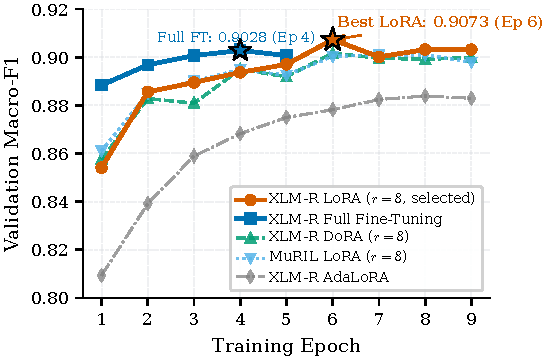
\includegraphics[width=\columnwidth]{figures/fig6_training_convergence.pdf}
\caption{Validation macro-F1 per epoch for XLM-R, seed 2024. Both curves flatten within about one point of each other.}
\label{fig:curve}
\end{figure}

\subsection{Rank, alpha and learning rate}
Table~\ref{tab:grid} shows the MuRIL grid (one seed). The whole grid spans about 1.5 points on validation, which is of the same order as seed-to-seed variation, so no single rank can be called best with confidence. Alpha~$=64$ was best at every rank. A learning rate of $10^{-4}$ under-trained (validation 0.8922) and $5\times10^{-4}$ degraded training (0.8438), against 0.9048 at $2\times10^{-4}$.

\begin{table}[t]
\caption{Validation macro-F1 on MuRIL for LoRA rank $r$ and scaling factor $\alpha$ (learning rate $2\times10^{-4}$, 10 epochs, one seed). Bold marks the best cell.}
\label{tab:grid}
\centering
\footnotesize
\begin{tabular}{lccc}
\toprule
 & $\alpha=16$ & $\alpha=32$ & $\alpha=64$ \\
\midrule
$r=4$  & 0.8896 & 0.8978 & 0.9002 \\
$r=8$  & 0.8915 & 0.8978 & \textbf{0.9048} \\
$r=16$ & 0.8982 & 0.8957 & 0.9006 \\
$r=32$ & 0.8944 & 0.8973 & 0.9019 \\
\bottomrule
\end{tabular}
\end{table}

\subsection{Significance}
Table~\ref{tab:sig} and Fig.~\ref{fig:forest} compare the selected XLM-R LoRA model with each alternative on the same test comments. Against full fine-tuning the interval includes zero for all three seeds (McNemar $p$ between 0.24 and 0.87), and the same holds for DoRA, MuRIL LoRA, MuRIL full fine-tuning, IndicBERT v2, the published recipe and the TF-IDF baseline. AdaLoRA is worse by 0.016 macro-F1 ($p=0.0002$). mBERT is worse with an interval that just excludes zero but a McNemar $p$ of 0.054. A seed-level Welch test of LoRA against full fine-tuning gives $p=0.47$ with three seeds per arm, which has little power. The test set of 2,997 comments cannot resolve differences much below one point, so the supported statement is non-inferiority within about one point, not superiority.

\begin{table}[t]
\caption{Selected XLM-R LoRA (seed 2024) compared with each alternative on the same 2,997 test comments. $\Delta$ is the macro-F1 of the selected model minus that of the alternative (positive favours the selected model), with a 95\% paired bootstrap interval and the exact McNemar $p$-value. Alternatives not labelled with a seed use seed 2024. After Bonferroni correction for 11 comparisons ($\alpha=0.0045$), only AdaLoRA differs significantly.}
\label{tab:sig}
\centering
\footnotesize
\setlength{\tabcolsep}{3.5pt}
\begin{tabular}{lccc}
\toprule
Alternative & $\Delta$ & 95\% interval & $p$ \\
\midrule
XLM-R full, seed 2024 & $-0.0050$ & $[-0.0127,+0.0027]$ & 0.235 \\
XLM-R full, seed 42 & $-0.0009$ & $[-0.0091,+0.0074]$ & 0.872 \\
XLM-R full, seed 123 & $+0.0015$ & $[-0.0067,+0.0095]$ & 0.811 \\
XLM-R DoRA & $-0.0004$ & $[-0.0070,+0.0063]$ & 1.000 \\
MuRIL LoRA & $+0.0024$ & $[-0.0060,+0.0107]$ & 0.634 \\
MuRIL full & $-0.0007$ & $[-0.0097,+0.0080]$ & 0.941 \\
XLM-R LoRA, $r{=}4,\alpha{=}32$, 5 ep.\ \cite{kaunang2026indo} & $+0.0037$ & $[-0.0037,+0.0107]$ & 0.355 \\
IndicBERT v2 LoRA & $+0.0067$ & $[-0.0024,+0.0157]$ & 0.168 \\
TF-IDF + SVM & $+0.0013$ & $[-0.0084,+0.0110]$ & 0.840 \\
mBERT LoRA & $+0.0097$ & $[+0.0007,+0.0193]$ & 0.054 \\
XLM-R AdaLoRA & $+0.0160$ & $[+0.0077,+0.0244]$ & $<0.001$ \\
\bottomrule
\end{tabular}
\end{table}

\begin{figure}[t]
\centering
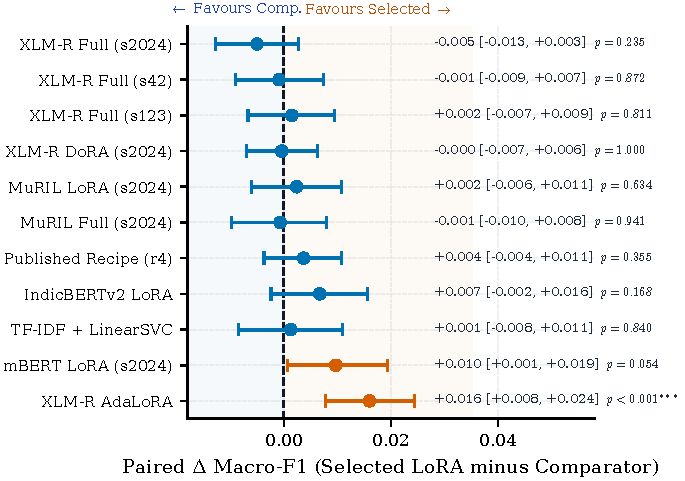
\includegraphics[width=\columnwidth]{figures/fig7_forest_significance.pdf}
\caption{Paired macro-F1 difference between the selected model and each alternative with 95\% bootstrap intervals (dashed line: no difference; right of zero favours the selected model). Only AdaLoRA, and marginally mBERT, are clearly separated.}
\label{fig:forest}
\end{figure}

\subsection{Expected versus observed outcomes}
Table~\ref{tab:expect} summarizes the expected and observed outcome for each model. Several expected benefits did not appear. AdaLoRA was expected to improve on uniform rank allocation, but it was the weakest method on both backbones and took about twice the training time of LoRA; an earlier run collapsed to chance level before its rank-allocation step was corrected, so this method is sensitive to implementation details. DoRA was expected to help especially at low rank, but gave a tie on XLM-R and a lower score on MuRIL. Indic-specific pretraining (MuRIL, IndicBERT v2) did not beat XLM-R. The published recipe transferred but scored 0.8985, about 0.5 points below the tuned setting; since rank, alpha, dropout, batch size, length and epoch budget all differ, the gap cannot be attributed to one factor, and two of three seeds of the $r=16$ configuration peaked on the last allowed epoch, which suggests that five epochs is short.

\begin{table*}[t]
\caption{Expectation against outcome for each model tested (test macro-F1, mean over three seeds except where noted). Verdicts: Met, Partly met, Not met. The SVM and INT8 rows are single runs.}
\label{tab:expect}
\centering
\footnotesize
\setlength{\tabcolsep}{4pt}
\renewcommand{\arraystretch}{1.05}
\resizebox{\textwidth}{!}{%
\begin{tabular}{>{\raggedright\arraybackslash}p{2.6cm}>{\raggedright\arraybackslash}p{4.4cm}>{\raggedright\arraybackslash}p{5.6cm}>{\raggedright\arraybackslash}p{2.4cm}}
\toprule
Model & Expected & Observed & Verdict \\
\midrule
XLM-R full fine-tuning & Accuracy ceiling & 0.9057, tied with cheaper models & Met (as baseline) \\
XLM-R LoRA & Near full accuracy with 1--2\% of the weights \cite{kaunang2026indo} & 0.9035 with 0.32\% of the weights & Met \\
LoRA rank study & A clear best rank & Small rank effect; larger $\alpha$ gives the best cells (one seed) & Partly met \\
AdaLoRA & Better than LoRA \cite{zhang2023adalora} & 0.8891, worse ($p=0.0002$), 2$\times$ slower & Not met \\
DoRA & Better than LoRA \cite{liu2024dora} & 0.9055 on XLM-R (tie), 0.9005 on MuRIL (lower) & Not met \\
mBERT LoRA & Trails XLM-R & 0.8946, lowest LoRA backbone (borderline, $p=0.054$) & Met \\
IndicBERT v2 LoRA & Beats general models on Telugu & 0.9017, tied, no gain & Not met \\
MuRIL & Beats XLM-R on Telugu & Full / LoRA: 0.9049 / 0.9052 vs 0.9057 / 0.9035 for XLM-R, tied & Not met \\
Published recipe & Near optimal & 0.8985, lower but not significant ($p=0.355$); also 5 epochs & Partly met \\
TF-IDF + SVM & Floor well below transformers & 0.9029, statistically tied & Not met \\
INT8 export & Small loss \cite{jacob2018} & Per-tensor collapsed; per-channel loses 1.2 points & Partly met (after fix) \\
\bottomrule
\end{tabular}}
\end{table*}

\subsection{Comparison with the classical baseline}
The TF-IDF and linear SVM model reaches 0.9029 test macro-F1 with a 30.3~MB file and a median latency of 1.65~ms per comment on one CPU thread, and it is statistically indistinguishable from the selected model ($p=0.84$). On this corpus, therefore, the transformers do not buy accuracy; the finding of this study is that adapting them cheaply costs no accuracy. It was not tested whether transformers help on implicit abuse, unseen vocabulary or code-mixed text, which is where an advantage would be expected.

\subsection{Robustness to disguised text}
Seven sentence-level and thirteen per-word disguises (spacing, zero-width characters, repeated letters, emoji, leetspeak, star-censoring, case) were applied to 600 test comments. Without the input guard every system falls to a mean accuracy of about 0.71 (Table~\ref{tab:rob} and Fig.~\ref{fig:rob}). With the guard, all three systems reach 0.86, so the gain comes from the guard and not from the model. Star-censored words (about 0.55) and combined letter repetition with zero-width characters remain weak points for all systems.

\begin{table*}[t]
\caption{Accuracy on 600 test comments under 20 disguise attacks, with and without the input guard. Mean and worst are taken over the 20 attacks (clean row excluded). LoRA and full fine-tuning rows use seed 2024.}
\label{tab:rob}
\centering
\scriptsize
\setlength{\tabcolsep}{4pt}
\renewcommand{\arraystretch}{0.95}
\resizebox{\textwidth}{!}{%
\begin{tabular}{llccc}
\toprule
Model & Guard & Clean & Mean attack & Worst attack \\
\midrule
TF-IDF + SVM & No  & 0.910 & 0.712 & 0.450 \\
             & Yes & 0.910 & \textbf{0.863} & \textbf{0.560} \\
\midrule
XLM-R full   & No  & 0.907 & 0.710 & 0.455 \\
             & Yes & 0.907 & 0.860 & 0.550 \\
\midrule
XLM-R LoRA   & No  & 0.897 & 0.725 & 0.458 \\
             & Yes & 0.898 & 0.856 & 0.552 \\
\bottomrule
\end{tabular}}
\end{table*}

\begin{figure}[t]
\centering
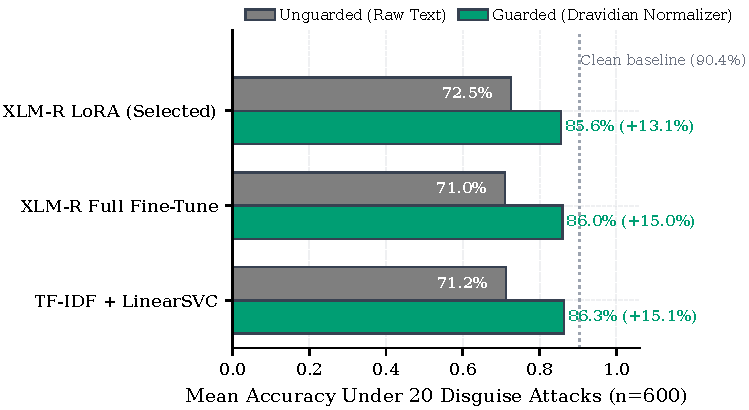
\includegraphics[width=\columnwidth]{figures/fig8_robustness_defense.pdf}
\caption{Mean accuracy under disguise attacks. The three guarded systems (blue) are far above the unguarded ones (grey) and are indistinguishable from each other.}
\label{fig:rob}
\end{figure}

Table~\ref{tab:attacks} breaks the robustness result down by attack. The guard repairs zero-width characters and separators inside words almost completely, partly repairs letter spacing and repetition, and cannot help with star-censoring, which removes the letters themselves. Emoji-based disguises are the one place where the model matters: without any guard-related repair, the selected LoRA model keeps 0.89 to 0.90 accuracy when words are wrapped in emoji or followed by emoji spam, against 0.80 to 0.85 for TF-IDF and 0.82 to 0.84 for full fine-tuning. Both transformers use the same inference code, so this difference originates in the models; the reason why the adapted model is less sensitive to emoji was not investigated.

\begin{table*}[t]
\caption{Accuracy on 600 test comments for each attack. Each cell is accuracy without the input guard / with the input guard, on the same 600 comments. The first row is the unattacked comment set. Sentence-level attacks change the whole comment; word-level attacks change every word. Mean and worst are over the 20 attacks (clean row excluded) and match Table~\ref{tab:rob}. LoRA and full fine-tuning use seed 2024.}
\label{tab:attacks}
\centering
\scriptsize
\setlength{\tabcolsep}{4pt}
\renewcommand{\arraystretch}{0.95}
\resizebox{\textwidth}{!}{%
\begin{tabular}{llccc}
\toprule
Level & Attack & TF-IDF + SVM & XLM-R full FT & XLM-R LoRA (selected) \\
\midrule
-- & None (clean) & 0.910 / 0.910 & 0.907 / 0.907 & 0.897 / 0.898 \\
\midrule
Sentence & Repeated chars (sentence) & 0.832 / 0.882 & 0.778 / 0.870 & 0.767 / 0.862 \\
Sentence & Extra spacing & 0.790 / 0.873 & 0.775 / 0.887 & 0.763 / 0.863 \\
Sentence & Emoji inserted & 0.892 / 0.892 & 0.902 / 0.902 & 0.902 / 0.903 \\
Sentence & Punctuation inserted & 0.893 / 0.895 & 0.908 / 0.908 & 0.897 / 0.897 \\
Sentence & Capitalization & 0.910 / 0.910 & 0.908 / 0.908 & 0.902 / 0.902 \\
Sentence & Number substitution & 0.903 / 0.905 & 0.912 / 0.912 & 0.890 / 0.893 \\
Sentence & Random case & 0.910 / 0.910 & 0.908 / 0.908 & 0.897 / 0.898 \\
\midrule
Word & Zero-width joiner & 0.688 / 0.910 & 0.455 / 0.907 & 0.458 / 0.898 \\
Word & Zero-width non-joiner & 0.450 / 0.910 & 0.455 / 0.907 & 0.458 / 0.898 \\
Word & Letter spacing & 0.608 / 0.835 & 0.455 / 0.845 & 0.458 / 0.765 \\
Word & Dots between letters & 0.477 / 0.893 & 0.508 / 0.902 & 0.480 / 0.890 \\
Word & Dashes between letters & 0.453 / 0.890 & 0.487 / 0.897 & 0.515 / 0.888 \\
Word & Emoji inside word & 0.460 / 0.892 & 0.655 / 0.900 & 0.758 / 0.905 \\
Word & Emoji wrapped around word & 0.800 / 0.800 & 0.818 / 0.818 & 0.890 / 0.892 \\
Word & Repeated chars (word) & 0.493 / 0.820 & 0.570 / 0.775 & 0.643 / 0.758 \\
Word & Leetspeak digits & 0.903 / 0.905 & 0.907 / 0.907 & 0.893 / 0.895 \\
Word & Star-censored & 0.558 / 0.560 & 0.550 / 0.550 & 0.552 / 0.552 \\
Word & Uppercase & 0.910 / 0.910 & 0.908 / 0.908 & 0.897 / 0.898 \\
Word & Trailing emoji spam & 0.852 / 0.852 & 0.837 / 0.837 & 0.900 / 0.902 \\
Word & Combined (repeat, zero-width, emoji) & 0.452 / 0.822 & 0.507 / 0.757 & 0.572 / 0.758 \\
\midrule
\multicolumn{2}{l}{Mean over 20 attacks} & 0.712 / 0.863 & 0.710 / 0.860 & 0.725 / 0.856 \\
\multicolumn{2}{l}{Worst attack} & 0.450 / 0.560 & 0.455 / 0.550 & 0.458 / 0.552 \\
\bottomrule
\end{tabular}}
\end{table*}

\subsection{Calibration, thresholds and deployment}
Temperature scaling ($T = 1.334$) reduces the expected calibration error of the selected model on validation from 0.035 to 0.013 and the Brier score from 0.0730 to 0.0711. With thresholds 0.45 and 0.50, the block decision has precision 0.928 and recall 0.897 on validation and sends 1.1\% of comments to human review. Table~\ref{tab:dep} shows the deployment variants. The INT8 export with per-channel weights loses about 1.2 points of test macro-F1 relative to FP32 and agrees with it on 96.8\% of test predictions. A per-tensor INT8 export of the MuRIL LoRA model made earlier in the study collapsed to 0.633 test macro-F1, and an INT8 file produced earlier in this project with the same per-tensor recipe scored 0.37 on a 600-comment sample; these failures would have gone unnoticed without evaluating the quantized model against FP32.

\begin{table*}[t]
\caption{Deployment variants of the selected XLM-R LoRA model (seed 2024; LoRA weights merged into the base model before export) and the TF-IDF + SVM baseline. Median latency per comment including tokenization, batch size one, on an Intel Core i7-13700 CPU (8 P-cores, 3.4 GHz, no GPU), with 1 and 4 CPU threads. The SVM runs single-threaded.}
\label{tab:dep}
\centering
\scriptsize
\setlength{\tabcolsep}{4pt}
\renewcommand{\arraystretch}{0.95}
\resizebox{\textwidth}{!}{%
\begin{tabular}{lccccc}
\toprule
Variant & Size (MB) & Val macro-F1 & Test macro-F1 & 1 thread (ms) & 4 threads (ms) \\
\midrule
FP32 merged (PyTorch)   & 1100 & 0.9073 & 0.9042 & 43.1 & 17.9 \\
INT8 ONNX, per-channel  & 279  & 0.8995 & 0.8926 & 23.1 & 8.3 \\
TF-IDF + SVM (baseline) & 30.3 & 0.8993 & 0.9029 & 1.65 & -- \\
\bottomrule
\end{tabular}}
\end{table*}

Figure~\ref{fig:calib} shows the reliability of the scores and the trade-off behind the thresholds. Before scaling, the model is over-confident: comments scored between 0.8 and 0.9 are right only 77\% of the time; after scaling, 82\%. Raising the block threshold trades recall for precision and sends more comments to review: at 0.70 the block precision is 0.950, recall 0.855 and 4.7\% of comments go to review; at 0.90 the figures are 0.984, 0.760 and 11.6\%. The chosen 0.50 keeps human review to about 1\% of traffic.

\begin{figure}[t]
\centering
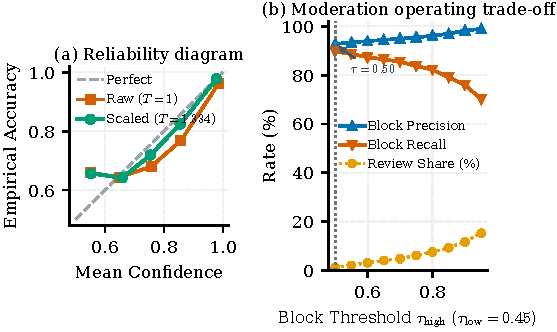
\includegraphics[width=\columnwidth]{figures/fig9_calibration_threshold_tradeoff.pdf}
\caption{Left: reliability on validation before and after temperature scaling (points on the dashed line are perfectly calibrated). Right: precision and recall of the block decision as the block threshold rises, with the review threshold fixed at 0.45.}
\label{fig:calib}
\end{figure}

\subsection{Template markers}
\label{sec:template_markers}
The seven Telugu marker strings that identify advertisement-like astrology and spell posts (with Romanized ISO 15919 transliteration) are:
\begin{enumerate}
    \item \textit{samasyalu} (problems / issues)
    \item \textit{etuvanti samasyakaina} (for any problem)
    \item \textit{sant\={a}nam} (progeny / children)
    \item \textit{bh\={a}ry\={a}bhartala} (husband and wife marital disputes)
    \item \textit{va\v{s}\={\i}kara\d{n}am} (love spell / vashikaran)
    \item \textit{pari\d{s}k\={a}ram} (guaranteed solution)
    \item \textit{c\={e}yaba\d{d}unu} (will be done / resolved)
\end{enumerate}

\subsection{Lessons for practitioners}
Three problems in this project changed the conclusions until they were found. First, an earlier run of LoRA with learning rate $10^{-4}$, three epochs and no early stopping gave 0.868 test macro-F1 on MuRIL and suggested that PEFT trails full fine-tuning by about four points; with learning rate $2\times10^{-4}$ and up to ten epochs the gap disappeared. Second, AdaLoRA first collapsed to 0.34 macro-F1; its rank-allocation step had never been called during training and its schedule was hard-coded, and fixing both (together with the new learning-rate setting) restored it to 0.89. Third, the per-tensor INT8 export scored 0.37 to 0.63 while looking like a normal model file. In each case the remedy was the same: compare against a trusted reference before drawing a conclusion. A short learning-rate and epoch search, a check that method-specific training hooks run, and an accuracy check of every exported model are cheap and would have prevented all three.

\subsection{Threats to validity}
The study uses one dataset in one language and a single test set of 2,997 comments. Three seeds give only coarse variance estimates, and the rank, alpha and learning-rate searches used one seed on MuRIL. Hyperparameters tuned for LoRA were reused for DoRA and AdaLoRA, which may understate them. Robustness was measured on 600 comments with synthetic disguises and may not reflect real attacks. Latency was measured on a desktop PC and not on low-end laptops, and peak RAM was not measured. Comments contain real abusive text; the corpus labels are those of the source dataset and were not re-annotated.

\subsection{Ethical considerations and reproducibility}
The system is meant to assist human moderators, not to replace them: the review band exists because about one test comment in ten is misclassified and false positives on critical or political speech carry real costs. The corpus contains real abusive text, which was used only as released, without new annotation or contact with users; examples are not reproduced in this paper. For reproducibility, every configuration was run with fixed seeds, all per-run metrics, training logs and confusion matrices were kept, and the selection rule is fully specified (Algorithm~\ref{alg:select}). The study needs one 8~GB consumer GPU; the 50 training runs of the study took about 12.6 hours of training time in total.

\section{Conclusion and Future Work}
\label{sec:concl}
On Telugu abusive comment detection, LoRA on the query and value matrices matches full fine-tuning within statistical noise while training under one percent of the parameters and using about a third of the GPU memory, so a 3.4~MB adapter can replace a 1.1~GB checkpoint. DoRA and AdaLoRA bring no benefit here, Indic-specific backbones do not beat XLM-R, and a TF-IDF and linear SVM baseline is as accurate on this corpus. The robustness measured here comes mostly from a simple input guard, although the adapted model is clearly less sensitive to emoji-based disguises. About 15\% of abusive comments are advertisement-like templates that inflate all scores, and 42\% of the selected model's errors are shared by every strong system. The most serious deployment error found was a silently broken INT8 export. Future work should evaluate on code-mixed and Romanized Telugu and on other domains where contextual models may help, tune DoRA and AdaLoRA separately, run more seeds and a larger test set, measure latency and memory on low-end laptops, test learned rather than rule-based defenses against disguised text, re-annotate the comments that every system misclassifies, and report scores with and without template posts.


%
% ---- Bibliography ----
%
\begin{thebibliography}{00}
%

\bibitem{kaunang2026indo} F. J. Kaunang, B. Hakim, and A. P. Thenata, ``Indonesian hate speech detection across diverse domains using parameter-efficient fine-tuning with IndoBERT and LoRA,'' \textit{Jurnal Minfo Polgan}, vol. 15, no. 2, 2026, doi:10.33395/jmp.v15i2.16581.
\bibitem{gupta2022macd} V. Gupta \textit{et al.}, ``Multilingual abusive comment detection at scale for Indic languages,'' in \textit{Advances in Neural Information Processing Systems 35, Datasets and Benchmarks Track}, 2022.
\bibitem{waseem2016} Z. Waseem and D. Hovy, ``Hateful symbols or hateful people? Predictive features for hate speech detection on Twitter,'' in \textit{Proc. NAACL Student Research Workshop}, 2016, pp. 88--93.
\bibitem{davidson2017} T. Davidson, D. Warmsley, M. Macy, and I. Weber, ``Automated hate speech detection and the problem of offensive language,'' in \textit{Proc. Int. AAAI Conf. Web and Social Media (ICWSM)}, vol. 11, no. 1, 2017, pp. 512--515.
\bibitem{schmidt2017} A. Schmidt and M. Wiegand, ``A survey on hate speech detection using natural language processing,'' in \textit{Proc. Fifth Int. Workshop on Natural Language Processing for Social Media}, 2017, pp. 1--10.
\bibitem{vaswani2017} A. Vaswani \textit{et al.}, ``Attention is all you need,'' in \textit{Advances in Neural Information Processing Systems 30}, 2017.
\bibitem{houlsby2019} N. Houlsby \textit{et al.}, ``Parameter-efficient transfer learning for NLP,'' in \textit{Proc. 36th Int. Conf. Machine Learning (ICML)}, PMLR vol. 97, 2019, pp. 2790--2799.
\bibitem{li2021prefix} X. L. Li and P. Liang, ``Prefix-tuning: Optimizing continuous prompts for generation,'' in \textit{Proc. 59th Annu. Meeting Assoc. Computational Linguistics (ACL)}, 2021, pp. 4582--4597.
\bibitem{lester2021prompt} B. Lester, R. Al-Rfou, and N. Constant, ``The power of scale for parameter-efficient prompt tuning,'' in \textit{Proc. Conf. Empirical Methods in Natural Language Processing (EMNLP)}, 2021, pp. 3045--3059.
\bibitem{aghajanyan2021intrinsic} A. Aghajanyan, S. Gupta, and L. Zettlemoyer, ``Intrinsic dimensionality explains the effectiveness of language model fine-tuning,'' in \textit{Proc. 59th Annu. Meeting Assoc. Computational Linguistics (ACL)}, 2021, pp. 7319--7328.
\bibitem{hu2022lora} E. J. Hu \textit{et al.}, ``LoRA: Low-rank adaptation of large language models,'' in \textit{Proc. Int. Conf. Learning Representations (ICLR)}, 2022.
\bibitem{zhang2023adalora} Q. Zhang \textit{et al.}, ``Adaptive budget allocation for parameter-efficient fine-tuning,'' in \textit{Proc. Int. Conf. Learning Representations (ICLR)}, 2023.
\bibitem{liu2024dora} S.-Y. Liu \textit{et al.}, ``DoRA: Weight-decomposed low-rank adaptation,'' in \textit{Proc. 41st Int. Conf. Machine Learning (ICML)}, PMLR vol. 235, 2024.
\bibitem{dettmers2023qlora} T. Dettmers, A. Pagnoni, A. Holtzman, and L. Zettlemoyer, ``QLoRA: Efficient finetuning of quantized LLMs,'' in \textit{Advances in Neural Information Processing Systems 36}, 2023.
\bibitem{liu2022ia3} H. Liu \textit{et al.}, ``Few-shot parameter-efficient fine-tuning is better and cheaper than in-context learning,'' in \textit{Advances in Neural Information Processing Systems 35}, 2022.
\bibitem{mangrulkar2022peft} S. Mangrulkar \textit{et al.}, ``PEFT: State-of-the-art parameter-efficient fine-tuning methods,'' 2022. [Online]. Available: \url{https://github.com/huggingface/peft}
\bibitem{conneau2020xlmr} A. Conneau \textit{et al.}, ``Unsupervised cross-lingual representation learning at scale,'' in \textit{Proc. 58th Annu. Meeting Assoc. Computational Linguistics (ACL)}, 2020, pp. 8440--8451.
\bibitem{khanuja2021muril} S. Khanuja \textit{et al.}, ``MuRIL: Multilingual representations for Indian languages,'' arXiv:2103.10730, 2021.
\bibitem{devlin2019bert} J. Devlin, M.-W. Chang, K. Lee, and K. Toutanova, ``BERT: Pre-training of deep bidirectional transformers for language understanding,'' in \textit{Proc. NAACL-HLT}, 2019, pp. 4171--4186.
\bibitem{doddapaneni2023indicbert} S. Doddapaneni \textit{et al.}, ``Towards leaving no Indic language behind: Building monolingual corpora, benchmark and models for Indic languages,'' in \textit{Proc. 61st Annu. Meeting Assoc. Computational Linguistics (ACL)}, 2023, pp. 12402--12426.
\bibitem{wolf2020transformers} T. Wolf \textit{et al.}, ``Transformers: State-of-the-art natural language processing,'' in \textit{Proc. EMNLP 2020: System Demonstrations}, 2020, pp. 38--45.
\bibitem{loshchilov2019adamw} I. Loshchilov and F. Hutter, ``Decoupled weight decay regularization,'' in \textit{Proc. Int. Conf. Learning Representations (ICLR)}, 2019.
\bibitem{cortes1995svm} C. Cortes and V. Vapnik, ``Support-vector networks,'' \textit{Machine Learning}, vol. 20, no. 3, pp. 273--297, 1995.
\bibitem{pedregosa2011sklearn} F. Pedregosa \textit{et al.}, ``Scikit-learn: Machine learning in Python,'' \textit{J. Machine Learning Research}, vol. 12, pp. 2825--2830, 2011.
\bibitem{sokolova2009} M. Sokolova and G. Lapalme, ``A systematic analysis of performance measures for classification tasks,'' \textit{Information Processing \& Management}, vol. 45, no. 4, pp. 427--437, 2009.
\bibitem{guo2017calibration} C. Guo, G. Pleiss, Y. Sun, and K. Q. Weinberger, ``On calibration of modern neural networks,'' in \textit{Proc. 34th Int. Conf. Machine Learning (ICML)}, PMLR vol. 70, 2017, pp. 1321--1330.
\bibitem{platt1999} J. C. Platt, ``Probabilistic outputs for support vector machines and comparisons to regularized likelihood methods,'' in \textit{Advances in Large Margin Classifiers}. Cambridge, MA: MIT Press, 1999, pp. 61--74.
\bibitem{efron1993bootstrap} B. Efron and R. J. Tibshirani, \textit{An Introduction to the Bootstrap}. New York: Chapman \& Hall, 1993.
\bibitem{mcnemar1947} Q. McNemar, ``Note on the sampling error of the difference between correlated proportions or percentages,'' \textit{Psychometrika}, vol. 12, no. 2, pp. 153--157, 1947.
\bibitem{dror2018} R. Dror, G. Baumer, S. Shlomov, and R. Reichart, ``The hitchhiker's guide to testing statistical significance in natural language processing,'' in \textit{Proc. 56th Annu. Meeting Assoc. Computational Linguistics (ACL)}, 2018, pp. 1383--1392.
\bibitem{dodge2020} J. Dodge \textit{et al.}, ``Fine-tuning pretrained language models: Weight initializations, data orders, and early stopping,'' arXiv:2002.06305, 2020.
\bibitem{zeiler2014} M. D. Zeiler and R. Fergus, ``Visualizing and understanding convolutional networks,'' in \textit{Proc. European Conf. Computer Vision (ECCV)}, 2014, pp. 818--833.
\bibitem{jacob2018} B. Jacob \textit{et al.}, ``Quantization and training of neural networks for efficient integer-arithmetic-only inference,'' in \textit{Proc. IEEE Conf. Computer Vision and Pattern Recognition (CVPR)}, 2018, pp. 2704--2713.
\bibitem{hosseini2017} H. Hosseini, S. Kannan, B. Zhang, and R. Poovendran, ``Deceiving Google's Perspective API built for detecting toxic comments,'' arXiv:1702.08138, 2017.
\bibitem{grondahl2018} T. Gr\"ondahl, L. Pajola, M. Juuti, M. Conti, and N. Asokan, ``All you need is `love': Evading hate speech detection,'' in \textit{Proc. 11th ACM Workshop on Artificial Intelligence and Security (AISec)}, 2018, arXiv:1808.09115.
\end{thebibliography}

\end{document}

